\subsection{Systems toxicology data set}
We dealt with a transcriptomics data set generated by leveraging data from a 6-month inhalation exposure study with ApoE-/- mice (Mus musculus) \cite{LoSasso2016TheReduction} \cite{Phillips2016AnCigarettes}, which reflects the effect of tobacco-based sources in the subjects against a control group (in a filtered-air environment). In addition to the control group, the study contains 5 exposure categories: cigarette smoke (CS) from the 3R4F reference cigarette, aerosol from the Carbon Heated Tobacco Product (CHTP), aerosol from the Tobacco Heating System (THS), switch from CS to a CHTP (SWITCH) and cessation of smoking (CESS). Each of them has testing time intervals of 3, 4, and 6 months.
\\

This information is available in a public repository \href{https://github.com/philipmorrisintl/MouseLungMultiOmics}{MouseLungMultiOmics - GitHub} provided by Philip Morris International \cite{Titz2020Multi-omicsSmoke}. Procedures of transcriptomics procurement are discussed within this work too.
\\

\subsection{External databases}
\label{section:external-db}
Computational Biology methods for Drug Discovery or \href{https://genestack.com/news/blog/case-study-clarivate-analytics/}{CBDD} \footnote{Clarivate Analytics: \url{https://genestack.com/news/blog/case-study-clarivate-analytics/}} database (Clarivate Analytics, Boston, MA) provides R-language API interface for information gathering. Interaction networks, gene full description and full pathways used in this work have been retrieved via R scripting access to the API.
\\

Assessing package’s components accuracy relies on CMAP2 lab-extracted data (Connectivity Map v.2 - The Broad Institute of MIT and Harvard in Cambridge, Massachusetts) \cite{Subramanian2017AProfiles} and TTD dataset (Therapeutic Target Database) \cite{Wang2020TherapeuticTherapeutics}.
Both resources are open source and available online.
\\

\subsection{Package structure}
As part of this work, we have built the R OMICS System Interpretation for R (\textit{omicssir}) package under the 3.5.1 version of RStudio. It is assembled in 5 modules or \textit{Cores}:
\\

\begin{itemize}
    \item Format Core (F) - Adapts lab-derived data to the algorithms.
    \item Operative Core (O) - Executes algorithms and (optionally) adds expansions.
    \item Benchmark Core (B) - Tests accuracy of the algorithms.
    \item Analysis Core (A) - Extracts biological insight from algorithm output. Includes figure and table plotting.
    \item Compare Core (C) - Under the same component, aims to find a consensus between algorithms, i.e. observe if their results match, based on different approaches and techniques but identical input.
\end{itemize}

\begin{figure}[!h]
    \centering
    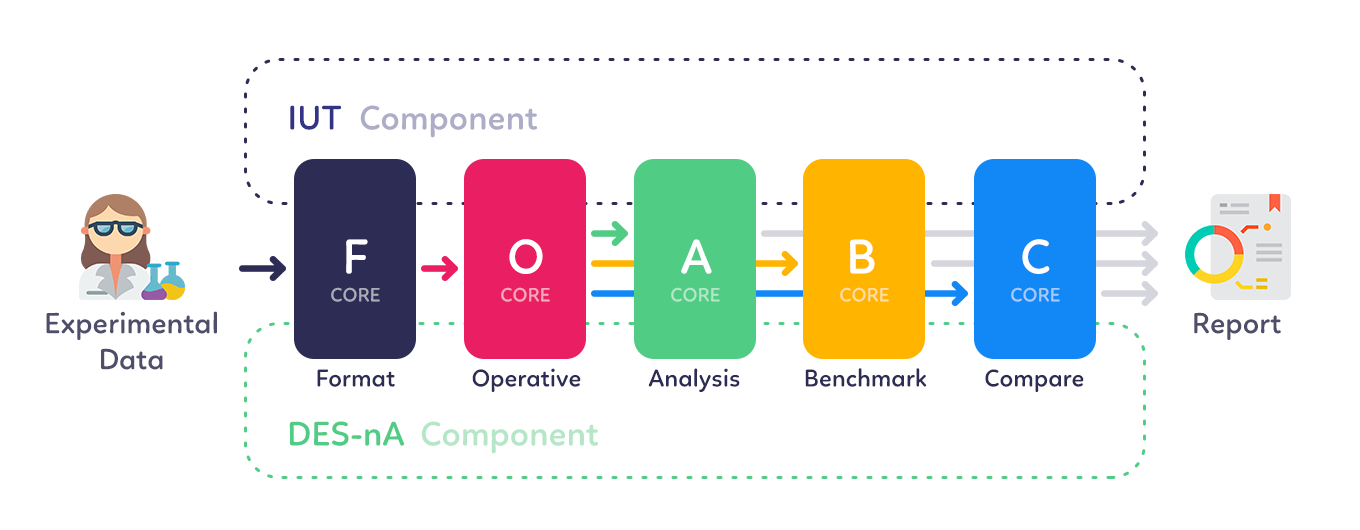
\includegraphics[width=\linewidth]{Major Thesis/figures/art/workflow.png}
    \caption{Package COREs distribution. Flow of information through the COREs is shown, from data obtaining to final report building.}
    \label{fig:workflow}
\end{figure}

We have named \textit{Component} each group of algorithms which share input format, algorithm operations, benchmark system and output information. Given their resemblance, their results are comparable under the \textit{Compare Core} to check for consensus in the delivered results.

In this project we group SigNet and MARINa algorithms into the Inference of Upstream Targets (IUT) component, and DEGAS and DIAMOnD into the Differential Expression Sub-network Analysis (DES-nA) component.

\subsection{Implementation}
A full run of the tool on transcriptomics data is done through an R Markdown file. It serves as a pipeline through the data and the entry of each algorithm (Figure \ref{fig:workflow}).

All dependencies have been resolved applying TidyVerse \footnote{Best practices guide: \url{https://style.tidyverse.org}} style guide in order to ensure maintainability and reproducibility in external environments.

\subsubsection{Inference of Upstream Targets - IUT Component}
The following algorithms aim to discover new targets among the transcription factors (TFs) which control the gene expression of an individual, based solely on the downstream reads. Results from this algorithms can aid in new drug design and also have a starting point where to focus on to lookup anomalies. SigNet and MARINa algorithms are part of this Component.

\paragraph{Format Core}
\label{section:iut-f}
Given a set of DE genes, they are cleaned for null values and then filtered using an absolute fold-change (FC) of 0.5 and an FDR-corrected p-value (Adj. p-value) of 0.05 to include only the relevant genes (based on literature).
\\

The CBDD's interface offers the MetaCore interaction network. We translate the gene symbols to MetaCore IDs. Since the molecular units and subunits can have colliding id numbers, after translation, duplicated FCs are clustered using mean as a default algorithm, keeping the same id.
\\

If a gene symbol cannot be found in the database, the Format Core relies on BioConductor limma package \footnote{\url{https://www.bioconductor.org/packages/release/bioc/html/limma.html}} to lookup synonyms and retry translation. Only 5\% of the genes could not be translated.
\\

SigNet’s input object is formatted to include the metabase\_id, FC and the original entrez\_gene\_id.
\\

Within the molecular interaction network from MetaCore, the majority of interactions (edges) are tagged as “Binding” or “Transcription Regulator” (Suppl. Material - Figure \ref{img:suppl:degrees}). The network is cropped to include only edges marked as “Transcription regulator”.

\paragraph{Operative Core}
SigNet uses the MetaCore network to calculate and infer the upstream regulators (URs) using causal graph theory and consensus ranking systems. Specific parameters of the original algorithm are set for the run based on literature: The maximum number of steps to consider a node unreachable in the causal network building is set to 20 (1 step = 1 edge or node jump); The minimum number of hypothesis for each run must be higher than 2 in order to ensure starting. To avoid having poor predictions, the default has been set to 10 starting nodes.
\\
\begin{table}[!h]
\begin{tabular}{|l|l|l|l|l|l|l|l|}
\hline
  & hypothesis & direction & reachable & unreachable & in\_original & {[}scores…{]} & final\_rank \\ \hline
1 & 23479      & -         & 134       & 2           & TRUE         & …             & 1           \\ \hline
2 & -53        & +         & 132       & 4           & TRUE         & …             & 2           \\ \hline
… & …          & …         & …         & …           & …            & …             & …           \\ \hline
N & 1723       & 1         & 0         & 136         & FALSE        & …             & N           \\ \hline
\end{tabular}
\caption{SigNet ranked list of hypothesis.}
\label{tbl:signet_output}
\end{table}

SigNet’s functions have been enhanced by overriding some functions. The three main rankers lambda, power weights and exponential weights [Suppl. Methods] return a score for each hypothesis in the original implementation. The score calculates how much contribution has each node over each hypothesis. Originally, the sum of scores of each row resulted in the final score for a hypothesis. Therefore, the full row includes the contribution of each node. Rankers’ have been modified to individually return the contribution of each node over the hypothesis.
\\

SigNet’s original algorithm result consists of a ranked list of the full network where we have URs (Table 2), predicting the top genes responsible for the inputted DE profile. The final score is based on the reachability of each node within the causal graph, and its consensus score.
\\

The full output of the expanded SigNet includes a ranked list of hypotheses, the causal graph, contributions matrix and metadata (scoring systems and score consensus method).

\begin{table}[!h]
\centering
\begin{tabular}{|l|l|l|l|l|l|}
\hline
  & hypothesis & direction & regulons & pos\_DETOR & neg\_DETOR \\ \hline
1 & 23479      & -         & 134      & 2          & 1,346      \\ \hline
2 & -53        & +         & 132      & 4          & 1,254      \\ \hline
… & …          & …         & …        & …          & …          \\ \hline
N & 1024       & -         & 130      & 6          & 1,067      \\ \hline
\end{tabular}
\caption{MARINa ranked list of hypothesis.}
\label{tbl:marina_output}
\end{table}

Unlike SigNet, MARINa’s outputs only top URs. It does not rank the whole network due to its regulon-based nature, i.e. infers TF activity from the global transcriptional activation of its regulon, and the calculations crop the network, ruling out poor candidates (Table 3). 
However, the output format is adapted to match SigNet’s, in order to ease interpretation and comparison at analysis and comparison steps, respectively.

\paragraph{Analysis Core}
Algorithms are run over all (13) contrasts under the same parameters hence, for each algorithm individually, we build:

\begin{itemize}
    \item A side-to-side comparison using heat maps to display URs’ ranks. (Figure \ref{fig:heatmap-overview}). The rows collect the set of first 20 top-ranked hypothesis across contrasts.
    \item An annotation the top N DEG influencers using Go-terms (Table \ref{tbl:goterms}). The relation gene-term can be one-to-many, hence the larger the N parameter is set, the larger the table is.
\end{itemize}

The interaction sub-network of the DE influencer formed by nodes that contributed significantly in its score (Figure \ref{fig:graph-expansion}). The density of the graph depends on the level of contribution. Using the individual score for each contributor, we can calculate its contribution percentage and perform a cumulative sum from the highest contributor to the lowest, and then cut at a preferred threshold. 
\\

Therefore, expressing “50\% of the contribution” indicates the graph contains only the top contributors nodes whose contribution percentage add up to 50\% of the total. Setting the threshold to 100\% includes all the nodes whose score > 0.

\paragraph{Compare Core}
The top-ranked URs are checked based on table results, i.e. we make an intersection of the raw outputs at gene id level, and compare their ranks (Figure Z.1). This comparison is also made using heat maps based on the intersected output.
The size of the output is proportional to the overlap of the individual results, serving this as a double-check of the biological discoveries.

\paragraph{Benchmarking Core}
To ease comprehension, a summary of the process can be found below:
Obtain .CEL files from CMAP2. These contain transcriptomics expression values from cells treated with certain drugs.
\begin{enumerate}
    \item Convert .CEL files to the same format as our input used: a set of DE genes.
    \item Run SigNet and MARINa on the new set and obtain upstream regulators targets: the benchmark set.
    \item Obtain Therapeutic Target Database (TTD) tables with known targets for drugs: the gold standard.
    \item Assess benchmark set against gold standard.
\end{enumerate}

First, we programmatically obtain gene expression data from CMAP2 database. Second, for each cell treated under a drug experiment (mixing time periods, concentrations and cell lines), the FC is calculated using CBDD library, and we build the final input DataFrame whose format matches the output of the Format Core (\ref{section:iut-f}).

Procedure for treating .CEL files to convert them to the same input we need for our project is described in Suppl. Material \ref{section:suppl:bench}, in order to avoid losing focus of this workflow.
\\

After, both SigNet and MARINa are run over the CMAP2-derived data, under custom parameters. The steps this process follows is the same as for any data inputed:
Filtering at the Format Core, calculations at Operative Core and results gathering at the Analysis Core.
\\

As we aim for an extensive benchmarking, we set an iteration which uses different filtering thresholds: p-value minimum value starts at 0.005 and increases to 0.05, 0.01, 0.1 and 0.5. The minimum starting nodes are set to 1, 10, 25 and 50. Given 1991 available cases, and after analysis (Figure \ref{img:benchprogramma_histogram}) they are first filtered on the strictest parameters to ensure all the iterations use the same input: 50 minimum starting nodes and 0.0005 p-value. The benchmark results are calculated over a set of 61 test cases.
\\

Then, we programmatically gather the drug-target relation knowledge from the TTD and build the gold standard. For format reasons, and to ease match and name universalisation, CID codes are used for drugs, and gene symbols for genes. The translation is supported by limma package, which aids in gene translation and synonyms retrieval, and PubChem REST API [reference], whose main aim is to identify drugs by their name and synonyms.
\\

Last, we perform the assessment. Scoring SigNet is done by creating \textit{cutting thresholds}. SigNet ranks the full reachable network, therefore all the reachable genes are present in the result. Since both the activation (+) and repression (-) instances are present in the ranking, we consider only the top ranked one for the scoring, based on the fact that the gene has been identified regardless its influence.
\\

\subsubsection{Differential Expression Sub-Network Analysis - DES-NA Component}

This module focuses on constructing de novo sub-networks based on the input. Their approach differs due to the format of the input, although the aim stays the same. DEGAS and DIAMOnD algorithms belong to this Component.

\paragraph{Format Core}
Given the gene expression of multiple contrasts (including controls) in a single data frame, we build a list containing 3 main elements for each of the contrasts: (1) A matrix of gene expression across contrast[i] and controls, (2) a phenotypes vector indicating which columns from matrix contain contrasts and which the controls and (3) the interaction network on which to work.
The controls corresponding to each contrast are specified within the main input object dat. This object/file is built by several lists, attributes and R structures, where the main coordinator is the I (capital “i”).

The contrasts available in the dat file also include timepoints. Per each contrast, 3 different measures have been made on different time points: after 3, 4 and 6 months. If timepoints flag is activated, the Core treats each combination of contrast and time point as a different case. Conversely, if deactivated, all contrast’s cases will be associated, e.g. contrasts “3R4F 3m”, “3R4F 4m”,“CHS 4m” are collapsed in “3R4F” and “CHS”.

\paragraph{Operative Core}
\label{section:desna-o}
Both DEGAS and DIAMOnD first perform checks for nodes and network mismatch to avoid NULL results. They take an interaction network to base calculations on, since their de novo technique requires existing curated interactions from MetaCore.

For DEGAS, K is the parameter that requires most of the time to calculate. The Operative Core has side functions to estimate this parameter by using greedy search, i.e. setting the upper and lower bounds we accept and iterating on each. The performance of the estimator is increased due to the intrinsic heuristics of DEGAS (ExpandingGreedy by default) which, although they depend on K value, ensure termination. Based on experimental tries, we always set k to at least l+1. 
On the other hand, L parameter is set by default in literature to 20\% of the number of cases available in the matrix excluding controls.

DIAMOnD iterates N times over each seed. All parameters are set to default, and N is set to 200, as in literature. We aim to build a network based on p-value significance, the method for connectivity analysis is automatically and internally set to over-connectivity search.

\paragraph{Analysis Core}
The amount of subnetwork generations delivered varies depending on the input. Since each subnetwork has a confidence score (from 0 to 1, being 1 the highest confidence) and a p-value, we filter down the list of results using a score of 0.5 and p-value of 0.5.

The fold-change matrix for each case, is used in the graph representation as see in Figure X, detailing the kind of interaction (1 = activation, 0 = unknown, -1 = inhibition) and a colour cluster for dysregulation. Parameters for clustering include an absolute threshold for considering a node dysregulated, which is set to 1.5, and, based on the full matrix of cases that support the subnetwork generation, which percentage of the cases represent a node as dysregulated. E.g. JUN is dysregulated because in at least 50\% of the N cases it has been detected as dysregulated.


\paragraph{Compare Core}
Comparison of de novo structures aims only to strengthen the prediction power of the tools. Since both rely on graph-related algorithms which do not take biological interactions into account, this module can only deliver a consensus response between algorithms within the same time-point.


The implementation includes a simple overlap of edges and nodes of the compared sets. The display of results includes an adjustable threshold which allows the delivery of figures that contain at least a min\_overlap percentage.


\paragraph{Benchmarking Core}
Due to time constraints and technical problems within the company concerning server availability, this Core has remained unfinished.
The intended directions for it were gathering known pathways from previous literature as well as the data used for building them. Only studies which include references to data would have been taken into consideration. Some examples we had were [1] and [2], although datasets (containing fold-changes and interactions) available in the algorithms papers of DEGAS [3] and DIAMOnD [4] were a simple solution. 

The intended workflow would have been:
Predicting pathways on DEGAS and DIAMOnD using datasets described in literature and available online.
Since each dataset is labeled with a disease identifier, match this identifier to pathway names, building the gold standard. GSEABenchmarkeR and GSEABenchmarking packages seemed to provide support for name matching.
Get overlap percentage between prediction and gold standard to calculate accuracy.

\subsubsection{R Markdown file/Report}
One of the main aims of the project is to pass on all the derived knowledge back to the labs, in order to serve as feedback for the experiments and hopefully aid in further decisions.

Each R Markdown file allows the generation of PDF, HTML or Word files. As a particular case, HTML reports, if needed, include an interactive version for graphs an heat maps. This has been included due to the complexity of the data the study might work with. Overcrowded graphs use networkD3 package for highlighting, adding and deleting nodes, while large heat maps use d3heatmap package to highlight specific values. A flag for the interactive version is also available at the top.